\documentclass[12pt]{article}
\usepackage[italian]{babel}
\usepackage[utf8]{inputenc}
\usepackage{hyperref}
\usepackage{graphicx}
\usepackage{float}
\usepackage{listings}
\usepackage{indentfirst}
\usepackage{caption}
\usepackage{subcaption}

\title{QSVM for Sentiment Analysis}
\author{Mario Bifulco (881727)}
\date{UniTo, 2023/2024}

\begin{document}

\maketitle

\section{Disclamer}

The following file is not intended to be read by third parties, 
its purpose is to keep track of the work done during the thesis. 
For this reason, I will not edit the style of the writing and will present what I have done in Italian.

\section{Research questions}

Quali sono le finalità di questa tesi? A quali domande vorrei rispondere?

\paragraph{Le QPU sono valide per task di machine learning?} 
La promessa del quantum computing è quella di velocizzare problemi “difficili" su calcolatori classici.
Ad oggi il quantum adiabatic computing permette di risolvere problemi di ottimizzazione di natura quadratica.
I problemi di machine learning si possono quasi sempre ridurre all'ottimizzazione, 
è quindi possibile trarre \emph{vantaggi} dagli approcci quantistici?

La domanda in questo momento è ambigua, innanzitutto bisogna decidere su quale aspetto effettuare il confronto:
\begin{enumerate}
    \item Tempo di apprendimento
    \item Qualità della soluzione
    \item Semplicità nella riscrittura del problema
\end{enumerate}
Bisogna inoltre considerare che le attuali QPU sono estremamente limitate, 
quindi bisogna considerare anche \emph{problemi di scalabilità}.

Questo probetto di tesi prende in esame le macchine a vettori di supporto (SVM) in cui, per definizione, 
esiste un problema di ottimizzazione quadratico nell'apprendimento.

La scelta di questa architettura rispetto ad altre non è dovuta solo al naturale collegamento con i problemi ideali per le QPU,
le SVM si sono rivelate architetture molto versatili, inoltre è possibile dimostrare matematicamente che il meccanismo di attenzione dei Transformer è equivalente al processo di ottimizzazione del margine delle SVM.
Ottenere quindi buoni risultati potrebbe portare ad una prima implementazione dell'architettura Transformer su macchine quantistiche.

\section{Dataset}

La tesi si articola in una riscrittura su architettura quantistica delle SVM per il task di sentiment analysis (SentA).

Come dataset per il problema si è scelto \textsc{TweetEval}, nel sottoinsieme \textsc{Sentiment}.
Questo dataset contiene frasi di Twitter suddivise in tre split, train, validation e test, 
ogni esempio è etichettato con una delle tre classi (positivo, negativo, neutro).

Siccome le SVM sono classificatori binari gli esempi di classe neutra sono stati scartati, 
e tra i rimanenti è stata applicata una normalizzazione per avere una distribuzione delle classi uniforme.
Nota: le classi di \textsc{TweetEval} sono positiva (2) e negativa (0), 
per riportare agli standard utilizzati dalle SVM sono state trasformate in 1 (positiva) e -1 (negativa).

Una volta limato il dataset per gli scopi del progetto è stato necessario trasformare le frase in embedding,
questo perché le architetture di machine learning non sono in grado di elaborare direttamente il testo, ma occorre una rappresentazione numerica.

Una prima trasformazione è stata effettuata tramite l'utilizzo di SentenceBert, 
una architettura Transformer che permette di ottenere l'embedding di una frase.

Successivamente è possibile sperimentare con eltre forme di embedding quali ad esempio:
\begin{itemize}
    \item Un senso mediano estratto da Word2Vec. Word2Vec permette di associare un embedding per ogni parola, ed è stato dimostrato come sia possibile svolgere “aritmetica di base" sugli embedding.
    \item Embedding custom estratti a partire dalle caratteristiche della frase decise dallo sviluppatore
\end{itemize}

\paragraph{Dataset di test}
Per poter testare e visualizzare durante la fase di sviluppo sono stati creati due dataset di supporto.

\begin{figure}[H]
    \centering
    \begin{subfigure}{.49\textwidth}
      \centering
      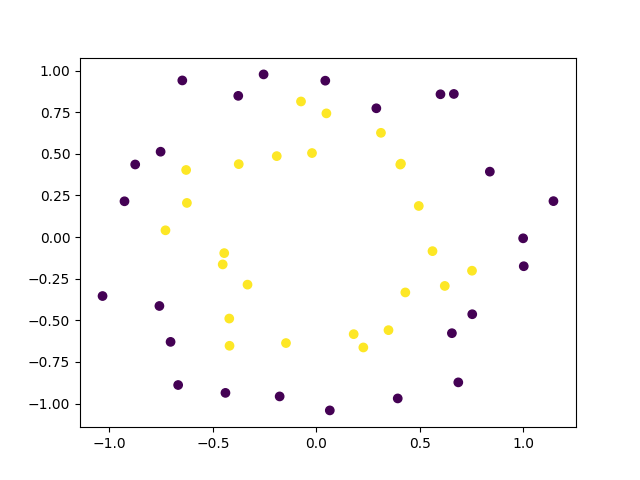
\includegraphics[width=\linewidth]{img/dummy.png}
      \caption{\textsc{Dummy} dataset}
    \end{subfigure}
    \begin{subfigure}{.49\textwidth}
      \centering
      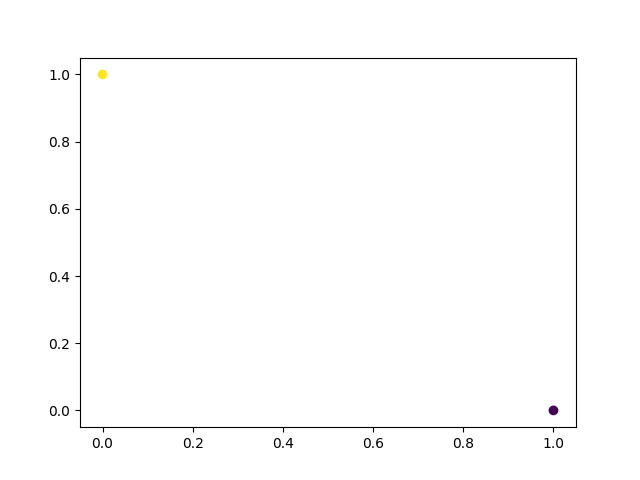
\includegraphics[width=\linewidth]{img/toy.png}
      \caption{\textsc{Toy} dataset}
    \end{subfigure}
\end{figure}

\section{Implementazione dell'architettura}



\section{Analisi del \emph{minor embedding}}

\end{document}